\documentclass[aspectratio=169]{beamer}

\usetheme{Madrid}
\usecolortheme{default}
\setbeamertemplate{navigation symbols}{}
\usepackage{graphicx}

\title{Booking Tool}
\subtitle{3-Hour Hackathon MVP}
\author{Hackathon Team}
\institute{Internal Equipment Reservation Tool}
\date{\today}

\begin{document}

\begin{frame}
  \titlepage
\end{frame}

\begin{frame}{Problem}
  \begin{itemize}
    \item Engineering and lab teams need a fast way to reserve shared equipment.
    \item Existing process is typically manual: chat, spreadsheet, or verbal coordination.
    \item This creates conflicts, poor visibility, and missing return tracking.
    \item Goal for the hackathon: deliver a usable MVP in 3 hours, not a production platform.
  \end{itemize}
\end{frame}

\begin{frame}{Hackathon Scope}
  \begin{itemize}
    \item Login with seeded users and one admin account.
    \item Browse equipment by category with live availability counts.
    \item Create reservation requests for a selected time window.
    \item Auto-assign a free physical unit from the chosen category.
    \item Admin workflow: approve, reject, confirm return, add equipment units.
    \item File-based persistence for deterministic local demos and tests.
  \end{itemize}
\end{frame}

\begin{frame}{Architecture}
  \begin{columns}[T]
    \begin{column}{0.52\textwidth}
      \begin{itemize}
        \item Single Next.js application with client UI and route handlers.
        \item React frontend fetches data from internal API endpoints.
        \item Domain logic is centralized in validation and DB helper modules.
        \item Persistence uses a JSON file seeded from a template.
        \item Design choice was driven by hackathon constraints: minimal setup, fast iteration, easy reset.
      \end{itemize}

      \vspace{0.5em}
      \textbf{Flow:} Browser $\rightarrow$ Next.js UI $\rightarrow$ API routes $\rightarrow$ validation $\rightarrow$ JSON DB
    \end{column}
    \begin{column}{0.44\textwidth}
      \centering
      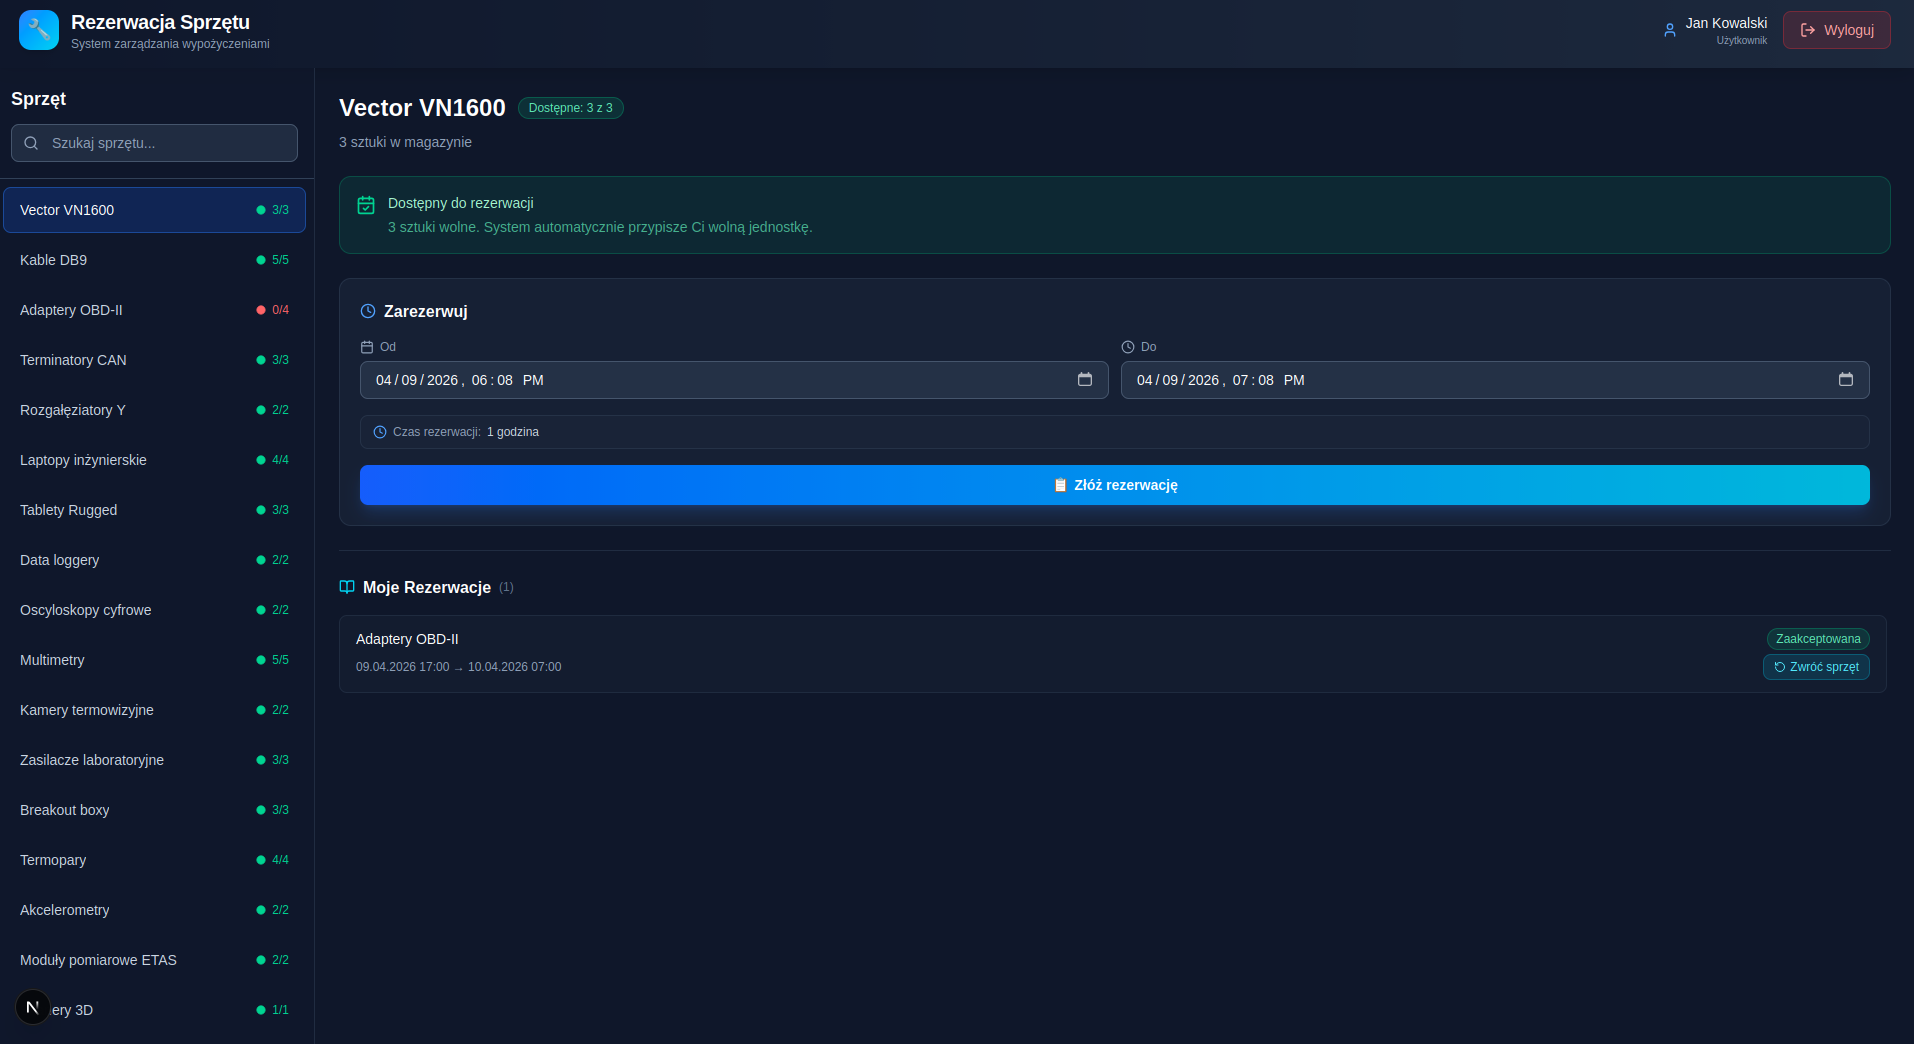
\includegraphics[width=\textwidth,height=0.52\textheight,keepaspectratio]{app screen.png}
    \end{column}
  \end{columns}
\end{frame}

\begin{frame}{Key User Flow}
  \begin{columns}[T]
    \begin{column}{0.5\textwidth}
      \begin{enumerate}
        \item User logs in.
        \item User selects an equipment category.
        \item User submits start and end time.
        \item Backend checks overdue items and slot conflicts.
        \item Backend finds a free unit in that category.
        \item Reservation is stored with \texttt{pending} status.
        \item Admin later approves or rejects the request.
      \end{enumerate}
    \end{column}
    \begin{column}{0.46\textwidth}
      \centering
      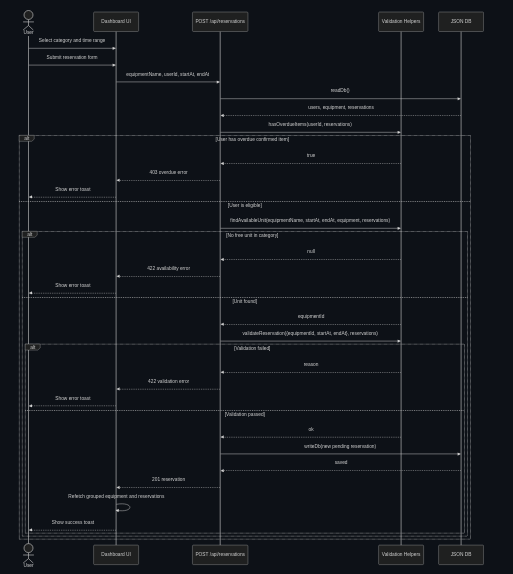
\includegraphics[width=\textwidth,height=0.55\textheight,keepaspectratio]{reservation sequence.png}
    \end{column}
  \end{columns}
\end{frame}

\begin{frame}{What The MVP Already Handles}
  \begin{columns}[T]
    \begin{column}{0.52\textwidth}
      \begin{itemize}
        \item Grouped equipment view with computed availability.
        \item Overlap detection per physical equipment unit.
        \item Blocking new reservations for users with overdue items.
        \item Reservation lifecycle: pending, confirmed, rejected, returned.
        \item Admin queue and active loan management from the same dashboard.
        \item Resettable local database for repeatable demos and end-to-end tests.
      \end{itemize}
    \end{column}
    \begin{column}{0.44\textwidth}
      \centering
      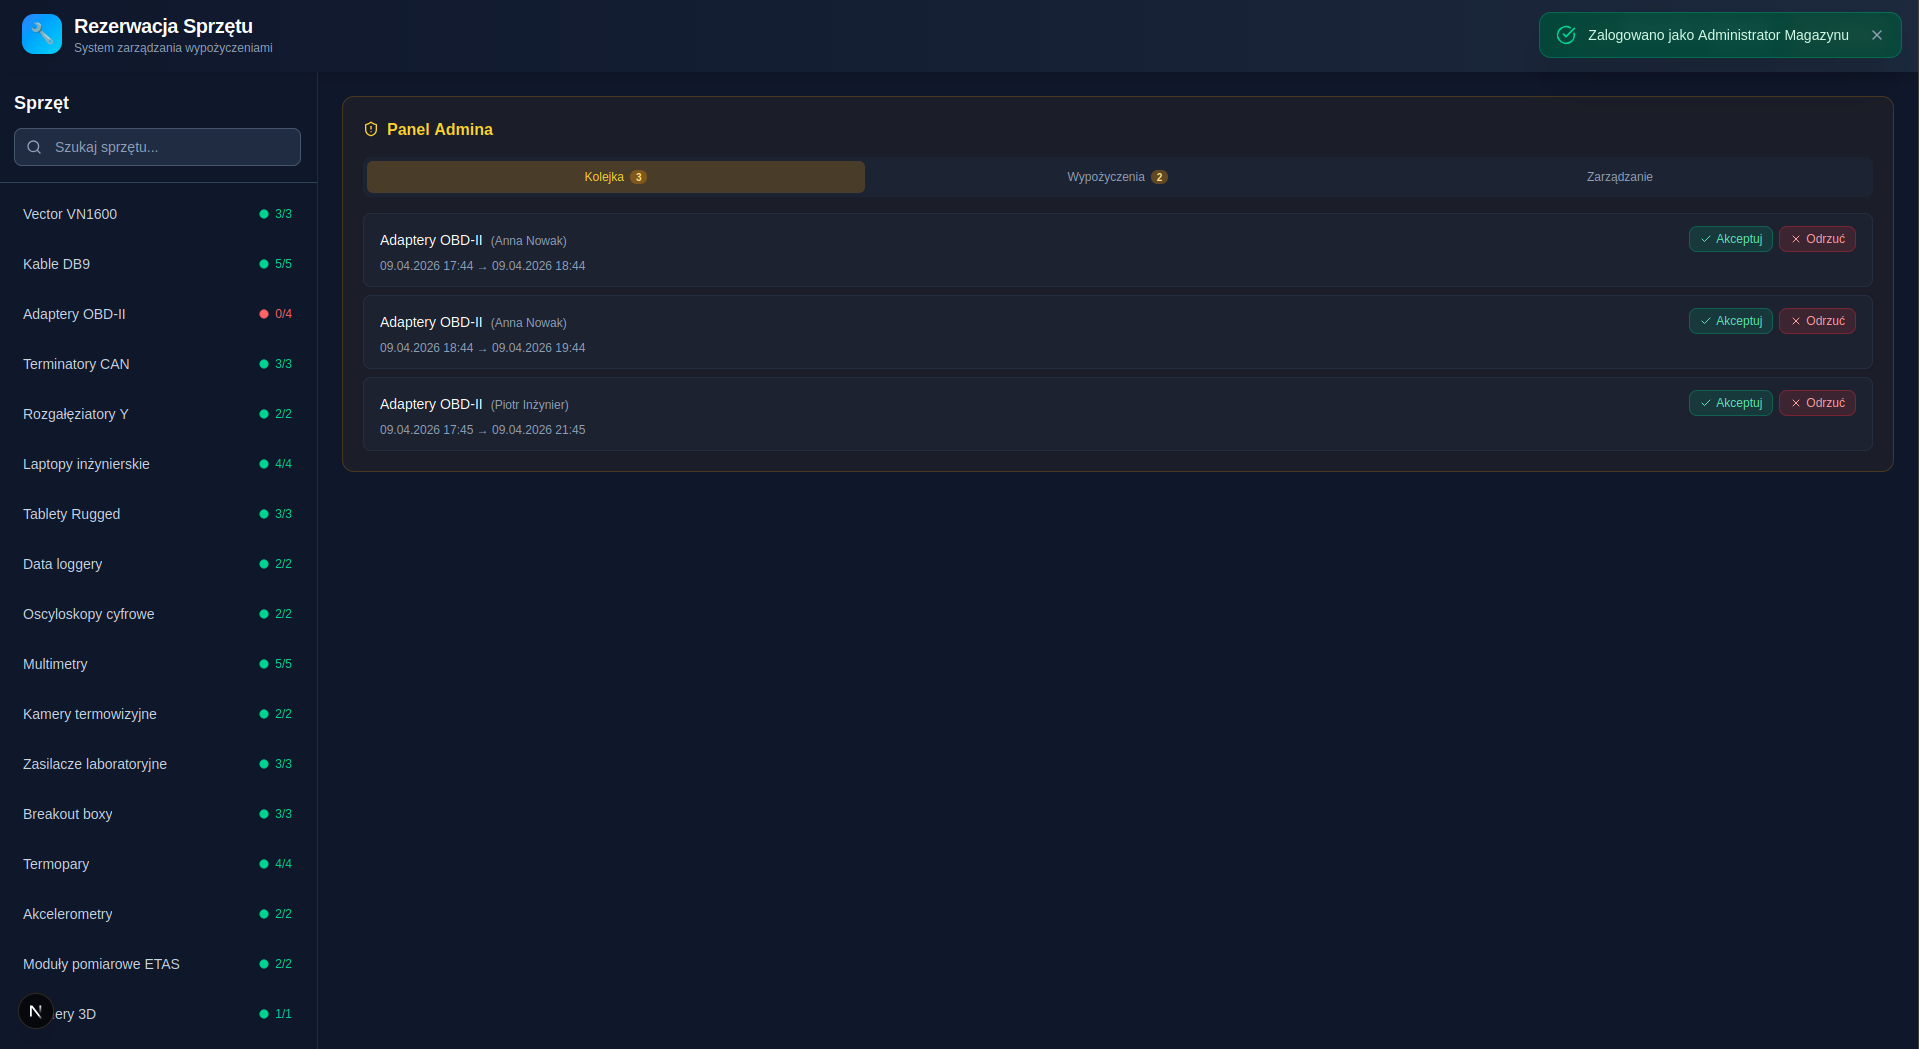
\includegraphics[width=\textwidth,height=0.5\textheight,keepaspectratio]{admin panel.png}
    \end{column}
  \end{columns}
\end{frame}

\begin{frame}{Tradeoffs For A 3-Hour Project}
  \begin{itemize}
    \item JSON file instead of a real database.
    \item No session or token-based authentication.
    \item Authorization is mostly enforced in the UI, not fully server-side.
    \item Single-app architecture instead of separated services.
    \item Optimized for clarity, speed, and demo readiness over scalability.
  \end{itemize}
\end{frame}

\begin{frame}{Testing And Demo Readiness}
  \begin{itemize}
    \item Unit and API tests cover validation and route behavior.
    \item Playwright covers end-to-end booking scenarios.
    \item Seeded users and reset scripts make the demo reproducible.
    \item Documentation includes architecture, use cases, and sequence diagrams.
    \item The demo can be reset quickly, which matters in a short hackathon presentation.
  \end{itemize}
\end{frame}

\begin{frame}{Next Steps Beyond The Hackathon}
  \begin{itemize}
    \item Add real authentication and server-side authorization.
    \item Move persistence from JSON files to a proper database.
    \item Add audit trail, reservation editing, and cancellation.
    \item Introduce notifications for approval, rejection, and overdue returns.
    \item Deploy with multi-user safety and concurrent write handling.
  \end{itemize}
\end{frame}

\begin{frame}{Summary}
  \begin{itemize}
    \item The project delivers a credible internal booking MVP within 3 hours.
    \item The solution is intentionally simple but functionally complete for a demo.
    \item Core value: clear reservation flow, admin control, and repeatable local setup.
  \end{itemize}
\end{frame}

\end{document}
